\section{Zielsetzung}
In diesem Versuch sollen die mikroskopischen Parameter untersucht werden
die die Bewegung von Leitungselektronen in Metallen beschreiben.\\
Dafür werden der elektrische Widerstand und die Hall-Spannung bei unterschiedlichen Materialien 
untersucht und dann ein Zusammenhang zwischen diesen Größen und Parametern wie der mittleren Driftgeschwindigkeit in Stromrichtung hergestellt.



\section{Theoretische Grundlagen}

\subsection{Bandstruktur und elektrische Leitfähigkeit von Kristallen}

In einem kristallinen Festkörper lassen sich die Energieniveaus seiner Elektronen und seine Leitfähigkeit durch
ein Modell mit Energiebändern beschreiben.\\
Die Valenzelektronen des Materials, also die Elektronen der äußersten Schale, 
bilden in einem kristallinen Festkörper ein zusammenhängendes System. Nach dem Pauli-Prinzip dürfen in einem System nur Elektronen mit entgegengesetztem Spin
den gleichen Zustand und damit gleiche Energie besitzen.\\
Die möglichen energetischen Zustände der Elektronen lassen sich dann, wie in Abb.\refeq{img:band} sichtbar,
durch quasikontinuierliche Energiebänder darstellen.\\
Die Lücken zwischen ihnen heißen \enquote{verbotene Zone} und bilden die nicht möglichen Zustände ab. 
Sie bilden oft eine Grenze zwischen den Bändern.
Es ist allerdings auch möglich, dass sich die Bänder überlappen.\\
Mit diesem Modell der Energiebänder lassen sich nun sehr gut Vorgänge, die die Elektronen des Festkörpers betreffen, beschreiben.\\
In einem komplett mit Elektronen gefülltem Band, wie es oft bei den Bändern der inneren 
Schalen der Fall ist, kann, da jeder mögliche Zustand besetzt ist,
kein Elektron Energie aufnehmen oder abgeben. \\
Durch einen dieser Prozesse würde das Elektron nämlich einen Zustand einnehmen müssen, der schon besetzt ist, was das Pauli-Prinzip untersagt.
Daraus folgt dann auch dass die Elektronen dieser Bänder nicht, zum Beispiel durch äußere elektrische Felder, beschleunigt werden können 
und damit nicht zur elektrischen Leitfähigkeit beitragen können.\\
Die Elektronen die beschleunigt werden können sind die, die in dem äußersten, nicht gefülltem Band sitzen.
In diesen Bändern gibt es Quantenzustände welche noch unbesetzt sind. Zum Beispiel die von Elektronen mit umgekehrtem Spin.
Die Elektronen in diesen Bändern haben also die Möglichkeit beschleunigt zu werden, wodurch sich in dem kristallinen Festkörper
ein makroskopischer Strom ausbilden kann.\\
Da dieser Strom durch Elektronen des nur teilweise besetzten Bandes hervorgerufen wird, werden sie auch Leitungselektronen und das Band das Leitfähigkeitsband genannt.\\\\

\begin{figure}[H]
  \centering
  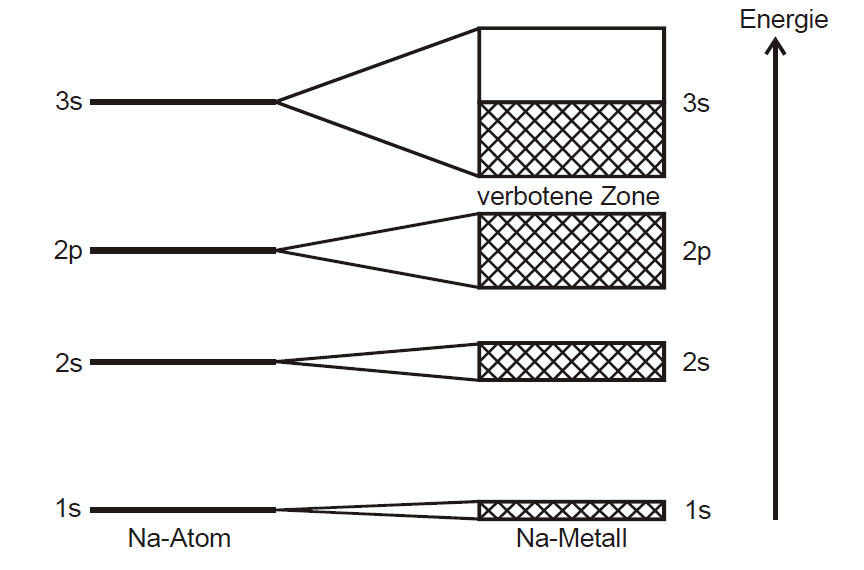
\includegraphics[width=0.55\textwidth]{images/energiebaender.PNG}
  \caption{Eine Darstellung der Energiebänder eines Natrium-Atoms \protect \cite{V311}.}
  \label{img:band}
\end{figure}

\noindent
Ein Beispiel dafür wären natürlich in erster Linie Metalle, die mit ihrer hervorragenden Leitfähigkeit, die sich nach diesem Prinzip beschreiben lässt, glänzen.\\
Ein anderes Beispiel ist in Abb.\refeq{img:band} in der die Bänder eines Natrium-Atoms aufgeführt sind zu sehen.\\
Die einzelnen sichtbaren Bänder sind dabei die einzelnen Schalen des Atoms.
Die Lücken zwischen ihnen sind dabei die zuvor genannten verbotenen Zonen.
Die 1s-, 2s-, 2p-, Bänder sind komplett gefüllt und tragen nichts zur elektrischen Leitfähigkeit bei.\\
Das 3s-Band, welches mit der 3s-Schale korrespondiert, ist allerdings nicht komplett gefüllt.
In der Schale befindet sich ein ungepaartes Elektron. Es ist also noch Platz für eins mit entgegengesetztem Spin.
Dadurch trägt dieses zur Leitfähigkeit bei.\\\\
\noindent
Bei nichtleitenden Festkörpern, oder auch Isolatoren, ist die verbotene Zone so breit, dass die Energie, 
die zum überspringen von ihr nötig wäre, nicht aufgebracht werden kann. Des Weiteren besitzt die äußerste Schale kein Elektron, welches
überhaupt erst beschleunigt werden könnte.\\\\
\noindent
Nach der Quantenmechanik sollten ideale Metallkristalle eine unendlich hohe Leitähigkeit besitzen, da
die Elektronen als Materiewellen betrachtet werden können, welche nicht in Wechselwirkung untereinander oder mit den Atomrümpfen treten.\\
Die endliche reale Leitfähigkeit lässt sich also auf Abweichungen vom Ideal und damit mit Fehlern im Kristallgitter begründen.\\


\subsection{Berechnung der Leitfähigkeit}

Die zuvor beschriebene Bewegung der Leitungselektronen durch das Kristallgitter lässt 
mit der Bewegung der Teilchen eines idealen Gases vergleichen.\\
Die Elektronen kollidieren mit Fehlstellungen im Gitter und auch mit Ionenrümpfen, die sich aus dem Gitterverband entfernt haben.
Sie werden, wenn ein elektrisches Feld anliegt, also nicht kontinuirlich beschleunigt sondern auch immer wieder in zufällige Richtungen gestreut.\\
Die Zeit zwischen solchen Zusammenstößen lässt sich über die mittlere Flugzeit $\overline{\tau}$ ausdrücken.\\
Während $\overline{\tau}$ wird, bei angelegtem Feld, ein Elektron also in Richtung $\vec{E}$ gleichmäßig beschleunigt.
Diese Beschleunigung lässt bei der Ladung $\symup{e_0}$\cite{e0} und der Ruhemasse des Elektrons $\symup{m_0}$\cite{m0} durch $\vec{b}$ ausdrücken.

\begin{equation}
  \vec{b} = -\frac{\symup{e_0}}{\symup{m_0}} \cdot \vec{E} \nonumber
\end{equation}
\noindent
Die Geschwindigkeitsänderung $\increment\vec{\overline{v}}$ während $\overline{\tau}$ in Richtung $\vec{E}$ ergibt sich dann zu:

\begin{equation}
  \increment\vec{\overline{v}}= -\frac{\symup{e_0}}{\symup{m_0}}\cdot \vec{E} \cdot \overline{\tau} 
  \label{eqn:v1}
\end{equation}
\noindent
Da die Elektronen, wie zuvor bereits erwähnt, immer zufällig gestreut werden, ändert sich immer ihre Geschwindigkeitskomponenten in Richtung
des elektrischen Feldes. Diese ist nach der Streuung, im Durchschnitt, immer null.
Nach jedem Stoß müssen die Elektronen also immer komplett neu in Richtung des elektrischen Feldes beschleunigt werden.\\
Dieser Sachverhalt lässt sich dann beschreiben in dem eine mittlere Driftgeschwindigkeit eingeführt wird, welche das Mittel aus $\increment\vec{\overline{v}}$ 
und 0 ist. Die Formel dafür ergibt sich dann zu:

\begin{equation}
  \vec{\overline{v_d}}=\frac{1}{2}\increment\vec{\overline{v}} 
  \label{eqn:v1}
\end{equation}
\noindent
Mit dieser Gleichung lässt sich sich dann eine Formel für die Stromdichte $j$ herleiten. Diese ist nämlich die Anzahl $n$ der Ladungen, hier ausgedrückt
über die Elektronenladung $-\symup{e_0}$, die sich mit dem Betrag der Geschwindigkeit $\overline{v_d}$ bewegen, also:

\begin{equation}
  j=-n\overline{v_d}\cdot \symup{e_0} 
  \label{eqn:j1}
\end{equation}
\noindent
Oder anders gesagt; Der Strom $I$, der durch die Querschnittsfläche des Drahtes $Q$ fließt, also $\frac{I}{Q}$.
Einsetzen von $\overline{v_d}$  führt dann zu:

\begin{equation}
  j=\frac{1}{2}n\frac{\symup{e_0}^2}{\symup{m_0}}\cdot \vec{E} \cdot \overline{\tau} \nonumber
\end{equation}
\noindent
Unter der Annahme, dass wir uns in einem homogenen Leiter befinden, lässt sich $j=\frac{I}{Q}$ und für das elektrische Feld $E=\frac{U}{L}$, wie im homogenen Feld eines Plattenkondensators, annehmen.
Erneutes einsetzen führt dann zu einer dem Ohm'schen Gesetz sehr ähnlichen Gleichung:

\begin{equation}
  I=\frac{1}{2}n\frac{\symup{e_0}^2}{\symup{m_0}}\cdot \overline{\tau} \frac{Q}{L} \cdot U
  \label{eqn:ohm1}
\end{equation}
Wenn nun \refeq{eqn:ohm1} mit dem Ohm'schen Gesetz $U=R\cdot I$ verglichen wird, wird sichtbar, dass 
\begin{equation}
  \frac{1}{R}=\frac{1}{2}n\frac{\symup{e_0}^2}{\symup{m_0}}\cdot \overline{\tau} \frac{Q}{L} = S\nonumber
\end{equation}
gelten muss.\\
Dieser Term, das Reziprok des Widerstands, wird als elektrische Leitfähigkeit $S$ bezeichnet. Wie aus \refeq{eqn:ohm1} ersichtlich bildet
sie einen Proportionalitätsfaktor zwischen Spannung und Strom.\\
Um allgemeinere Größen zu erhalten werden nun die geometrieabhängigen Größen $Q$ und $L$ weggelassen.\\
Dadurch wird $S$ zur spezifischen Leitfähigkeit $\sigma$ und $R$ wieder zu dem dazu reziproken spezifischen Widerstand $\rho$.
\begin{align}
  \sigma&=\frac{n}{2}\frac{\symup{e_0}^2}{\symup{m_0}}\cdot \overline{\tau}  \label{eqn:sigma}\\
  \rho &=\frac{2}{n}\frac{\symup{m_0}}{\symup{e_0}^2 \cdot \overline{\tau}}  \label{eqn:rho}
\end{align}



\subsection{Hall-Effekt}

Für die weitere Bestimmung von $I$ in \refeq{eqn:ohm1} fehlen noch die Variablen $n$ und $\overline{\tau}$.\\
Die Anzahl der Teilchen $n$ lässt sich einfach mit Hilfe des Hall-Effektes bestimmen.\\
Beim Hall-Effekt wird eine Spannung $U_H$, die an einer Metallplatte, in einem Magnetfeld, abfällt, gemessen.
Die Platte besitzt dabei die Maße, wie in Abb \refeq{img:hall} sichtbar, Breite $b$ und Dicke $d$.
Wenn sie nun in senkrecht in ein homogenes Magnetfeld gehalten wird und sie an eine Spannung angeschlossen wird, fließt ein Strom $I_q$ durch sie.
Wenn dann der Elektronenstrom durch die Platte und damit durch das Magnetfeld fließt werden sie duch die Lorentzkraft $F_L$ abgelenkt.\\
Dieser Aufbau ist schematisch in der unteren Abbildung \refeq{img:hall} dargestellt. Dort ist die Platte, die senkrecht im Magnetfeld liegt, 
an der ein Konstantstromgerät angeschlossen ist und das Voltmeter, welches die Hall-Spannung abgreift, zu sehen. 

\begin{figure}[H]
  \centering
  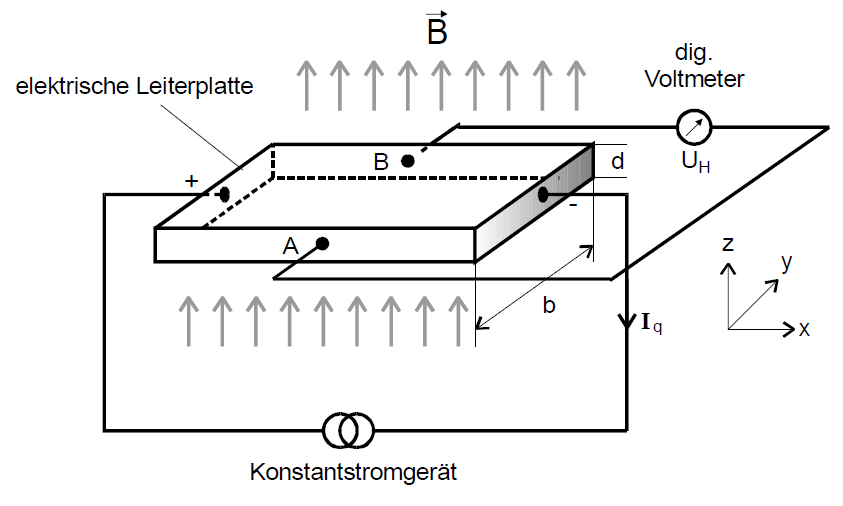
\includegraphics[width=0.55\textwidth]{images/hall.PNG}
  \caption{Die schematische Abbildung eines Aufbaus zur Messung des Hall-Effektes \protect \cite{V311}.}
  \label{img:hall}
\end{figure}

\noindent
Die Lorentzkraft hat bei orthogonaler Elektronenbewegung zum Magnetfeld, mit $B$ als Betragsstärke des Magnetfeldes und den anderen zuvor erklärten Variablen, den Betrag:
\begin{equation}
  F_L= \symup{e_0} \cdot \overline{v_d}B \nonumber
\end{equation}
Diese Kraft treibt die Elektronen dann an den Rand der Platte, wodurch sich dann eine Ladungsdifferenz zwischen den beiden Seiten der Platte ausbildet. 
Dies ist die bereits genannte Hall-Spannung $U_H$. Sie ist allerdings nicht nur von $F_L$ abhängig, da sich an den Rändern 
entgegenwirkend zur Lorentz-Kraft ein elektrisches Feld ausbildet. Bei konstantem Strom bildet sich dann dort ein Gleichgewichtszustand aus.
Deswegen gilt mit $U_H$ als Hall-Spannnung, $b$ als Breite der Platte und $\symup{e_0}$ als Betrag der Elementarladung, 
da bei der Lorentzkraft auch nur der Betrag betrachtet wurde:
\begin{equation}
  \symup{e_0} \cdot \overline{v_d}B =\symup{e_0} \cdot \frac{U_H}{b} \nonumber
\end{equation}
Umformen führt dann zu:
\begin{equation}
  U_H=b\overline{v_d}B
\end{equation}
Mit Hilfe der Gleichung \refeq{eqn:j1} lässt sich dann weiter umformen:
\begin{align}
  j&=\frac{I_q}{Q}=\frac{I_q}{bd}=-n \cdot \overline{v_d} \cdot bd\cdot \symup{e_0} \\
  \implies \overline{v_d} &= - \frac{I_q}{nbd\cdot \symup{e_0}}
  \intertext{Erneutes einsetzen:}
  \implies U_H&=- \frac{I_q \cdot B}{n\cdot d\cdot \symup{e_0}}\label{eqn:uhall}
\end{align}
Die ist nun die Formel mit der sich $n$ berechnen lässt.

\subsection{Berechnung der mikroskopischen Leitfähigkeitsparameter R und $\text{U}_\text{H}$} 

Für weitere Rechnungen ist die mittlere freie Weglänge $\overline{l}$ von Nöten.
Diese ist die die Strecke die ein Leitungselektron im Durchschnitt zwischen zwei Zusammenstößen zurücklegt. 
Sie ist dabei abhängig von der mittleren Flugzeit und der Totalgeschwindigkeit.
\begin{equation}
  \overline{l}= \overline{\tau} \cdot |v|
  \label{eqn:wegl}
\end{equation}
Die Totalgeschwindigkeit $|v|$ ist dabei die wirkliche Geschwindigkeit und nicht wie zuvor betrachtet  die relativ Geschwindigkeit.
Sie wird durch die thermische Energie der Teilchen hervorgerufen. Außerdem ist sie in der Regel auch deutlich höher als die Driftgeschwindigkeit.\\\\
\noindent
Wenn nun für die Elektronen wieder angewendet wird, dass sich die Atome wie die eines idealen Gases verhalten, lässt sich über das Äquipartitionstheorem
ihre mittlere Energie pro Freiheitsgrad bestimmen. Diese beträgt nämlich $\frac{\symup{k}\cdot T}{2}$ pro Freiheitsgrad mit T als Temperatur und 
$\symup{k}$ \cite{Boltzmann} als Boltzmann-Konstante.\\
Insgesamt ergibt sich das dann zu:
\begin{equation}
  E_\text{kin}=\frac{3}{2}\symup{k}\cdot T \nonumber
\end{equation}
Mit der klassischen Formel für die kinetische Energie lässt sich das ganze dann
durch gleichsetzen und umformen nach der mittleren Totalgeschwindigkeit $|\overline{v}_\text{kl}|$ zu
\begin{align}
  \overline{E}_\text{kin} &=\frac{\symup{m_0}}{2} \cdot |\overline{v}_\text{kl}|^2  \label{eqn:energ}\\
  \implies |\overline{v}_\text{kl}| &=\sqrt{\frac{3\symup{k}T}{\symup{m_0}}} \label{eqn:vtot}
\end{align}
umstellen.\\
Dabei ist $\symup{m_0}$ wieder die Elektronenruhemasse.\\
Allerdings lässt sich die Energie der Elektronen, aus dem zuvor genannten Grund des Pauli-Prinzips,
die Energieverteilung der Elektronen, nicht wie bei einem idealen Gas typisch, über die Maxwell-Boltzmann-Statistik darstellen.
Für diesen Fall wird dafür die Fermi-Dirac-Verteilung genutzt.\\
Sie beschreibt die Wahrscheinlichkeit $f(E)$ um ein Teilchen mit der Energie $E + \symup(d)E$ anzutreffen.
$E_F$ ist dabei die Fermi-Energie. Dies ist die Energie welche die energiereichsten Elektronen am absoluten Nullpunkt besitzen.
Sie ist dabei abhängig von der Dichte der Elektronen, dem Planck'schen Wirkungsquantum \cite{Planck} $\symup{h}$ und wieder der Elektronenmasse.\\
\begin{align}
  f(E)\symup{d}E &= \frac{1}{\symup{e}^{\frac{E-E_F}{\symup{k} \cdot T}}+1} \symup{d}E \label{eqn:fermidirac}\\
  E_F &= \frac{\symup{h}^2}{2 \cdot \symup{m_0}}\sqrt{\left(\frac{3}{8\pi}\right)^2} \label{eqn:E_F}
\end{align} 
Die beiden Formeln werden auch noch mal in der Grafik \ref{img:fermi} veranschaulicht.
Dort ist die Wahrscheinlichkeitsverteilung für die Elektronen dargestellt. 
Dabei ist die Energie $E_F$ besonders hervorgehoben.
Die gestrichelte Linie zeigt die Verteilung bei $T=0$ und die durchgezogene für $T>0$.

\begin{figure}[H]
  \centering
  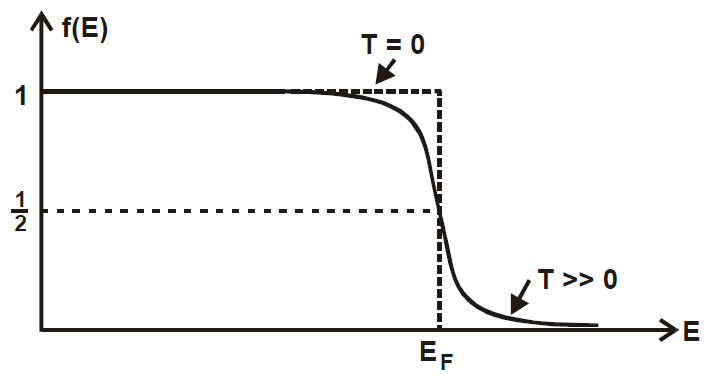
\includegraphics[width=0.55\textwidth]{images/dirac.PNG}
  \caption{Ein Diagramm der Fermi-Dirac-Verteilung. Die Abweichung zwischen dem gestrichelten Graphen für $T=0$ 
  und dem durchgezogenen für $T>0$ sind übertrieben dargestellt.  \protect \cite{V311}.}
  \label{img:fermi}
\end{figure}

\noindent
Die Formel \refeq{eqn:energ} lässt sich nun mit der Formel \refeq{eqn:E_F} annähern.\\
Denn es gilt  $ E\approx E_F$, da hauptsächlich nur die Elektronen mit diese Energie durch das Feld beschleunigt werden können.
Der Rest hat kleinere Energien und kann wegen des Pauli-Prinzips nicht beschleunigt werden.\\
Der zuvor gewählte Ansatz aus \refeq{eqn:vtot} mit der reinen thermischen Energie für die Totalgeschwindigkeit ist hier also in der Form, für die interessanten Elektronen, nicht anwendbar.
Die Totalgeschwindigkeit lässt sich also zu 
\begin{equation}
  |\overline{v}| \approx \sqrt{\frac{2E_F}{\symup{m_0}}} \nonumber
\end{equation}
approximieren.\\
Einsetzen dieser Gleichung in \refeq{eqn:wegl} führt dann zu einer Formel für die mittlere freie Weglänge:
\begin{equation}
  \overline{l} \approx \overline{\tau} \sqrt{\frac{2E_F}{\symup{m_0}}} \nonumber
\end{equation}
Das $\overline{\tau}$ lässt sich über die Gleichung \refeq{eqn:ohm1} bestimmen.\\
Des Weiteren lässt sich aus $\overline{\tau}$ auch noch die Beweglichkeit $\mu$ berechenen. Dafür wird Formel \refeq{eqn:v1} in \refeq{eqn:v1} eingesetzt.
\begin{align*}
  \vec{\overline{v_d}}&=-\frac{1}{2}\frac{\symup{e_0}}{\symup{m_0}}\cdot   \overline{\tau} \cdot \vec{E}\\
  \vec{\overline{v_d}}&= \mu \cdot \vec{E} & &\text{mit} & \mu&= -\frac{1}{2}\frac{\symup{e_0}}{\symup{m_0}}\cdot   \overline{\tau}\\
\end{align*}


%Braucht man die beweglichkeit $\my}$???????\\
%Wenn ja [insert here]


\subsection{Elektrizitätsleitung mit positiven Ladungsträgern}

Obwohl Elektronen die einzigen Teilchen sind, die sich im Kristallgitter bewegen können, kann es auch zu einer Art Bewegung positiver Ldungen kommen.
Dabei bewegen sich keine Ionen, sondern Ladungslöcher, also Leerstellen an denen normalerweise Elektronen sitzen sollten.\\
Dies kann zum Beispiel bei zweiwerigen Metallen, also Metallen die zwei Wasserstoffatome binden könnten, vorkommen.
Dort können sich nämlich die Energiebänder überlappen, so dass Elektronen aus den unteren Bändern einfach in das obere übergehen können und so 
dann Lücken hinterlassen.\\
Diese Löcher können sich frei bewegen und werden als positive Ladungen behandelt. Analog zum Elektron beeinflussen sie die Leitfähigkeit und erzeugen
eine entegengerichteten Hall-Effekt, den anomalen Hall-Effekt.\\
Allerdings muss für die Löcher mit anderen Massen und anderen Beweglichkeiten gerechnet werden.





